\textit{Pour chacune des affirmations suivantes, indiquer si elle est vraie ou fausse. Chaque réponse doit être justifiée. Une réponse non justifiée ne rapporte aucun point.}

\smallskip

\begin{enumerate}
	\item On considère ci-dessous la tableau de variations d'une fonction $f$ définie sur $\R \backslash\{-2\}$.
	
	\begin{Centrage}
		\begin{tikzpicture}[double distance=2pt]
			\tkzTabInit{$x$/1,$f$/2}{$-\infty$,$-2$,$1$,$+\infty$}
			\tkzTabVar{+/$5$,-D-/$-\infty$/$-\infty$,+/{3},-/$1$}
		\end{tikzpicture}
	\end{Centrage}
	\begin{enumerate}
		\item \textbf{Affirmation 1 :}
		
		La droite d'équation $y=-2$ est asymptote horizontale à la courbe $\mathcal{C}_f$ de la fonction $f$.
		\item \textbf{Affirmation 2 :}
		
		$\lim\limits_{x \to -\infty} \dfrac{2}{f(x)-5} = +\infty$.
	\end{enumerate}
	\item On considère la fonction $g$ définie sur $\R$ par $g(x)=x\,\e^{-x}$.
	\begin{enumerate}
		\item \textbf{Affirmation 3 :}
		
		Le point $A\left(2;\frac{2}{\e^2}\right)$ est l'unique point d'inflexion de la courbe $\mathcal{C}_g$ de la fonction $g$.
		\item \textbf{Affirmation 4 :}
		
		Pour tout nombre réel $x$ appartenant à $\IntervalleOO{-\infty}{2}$, on a : $g(x) \leqslant x$.
	\end{enumerate}
	\item \textbf{Affirmation 5 :}
	
	L'équation $x\,\ln(x)=1$ admet exactement deux solutions sur l'intervalle $\IntervalleOO{0}{+\infty}$.
\end{enumerate}